\documentclass[journal]{IEEEtran}

\usepackage{blindtext}
\usepackage{algorithm}
\usepackage{algorithmic}
\usepackage{cite}
\usepackage{graphicx}
\usepackage{array}
\usepackage{color}
\usepackage{tabularx}
\usepackage{epsfig}
\usepackage{amsmath}
\usepackage{amssymb}
\usepackage{bm}
\usepackage{wasysym}
\usepackage{circuitikz}
\usepackage{float}
\usetikzlibrary{arrows,shapes,calc,positioning}

\newcommand{\myscope}[2]
{\draw[thick,rotate=#2] (#1) circle (12pt)
(#1) ++(-0.35,-0.1) --++ (0.3,0.3) --++ (0,-0.3) --++(0.3,0.3) --++(0,-0.3);}

\begin{document}

\title{CSCE 221 \\ Checkpoint 4 Revision}

\author{Jacob~Purcell,~\IEEEmember{Texas~A\&M,~Student}}

\maketitle


\subsection*{Problem 3}

The first submission did not answer part b. Although the algorithm may be optimized by having
the queue reload itself (using size() to keep track of position), the previous algorithm will be analyzed for 
time complexity. $Q1, Q2$ will be used as predeclared queues.

\begin{figure}[H]
    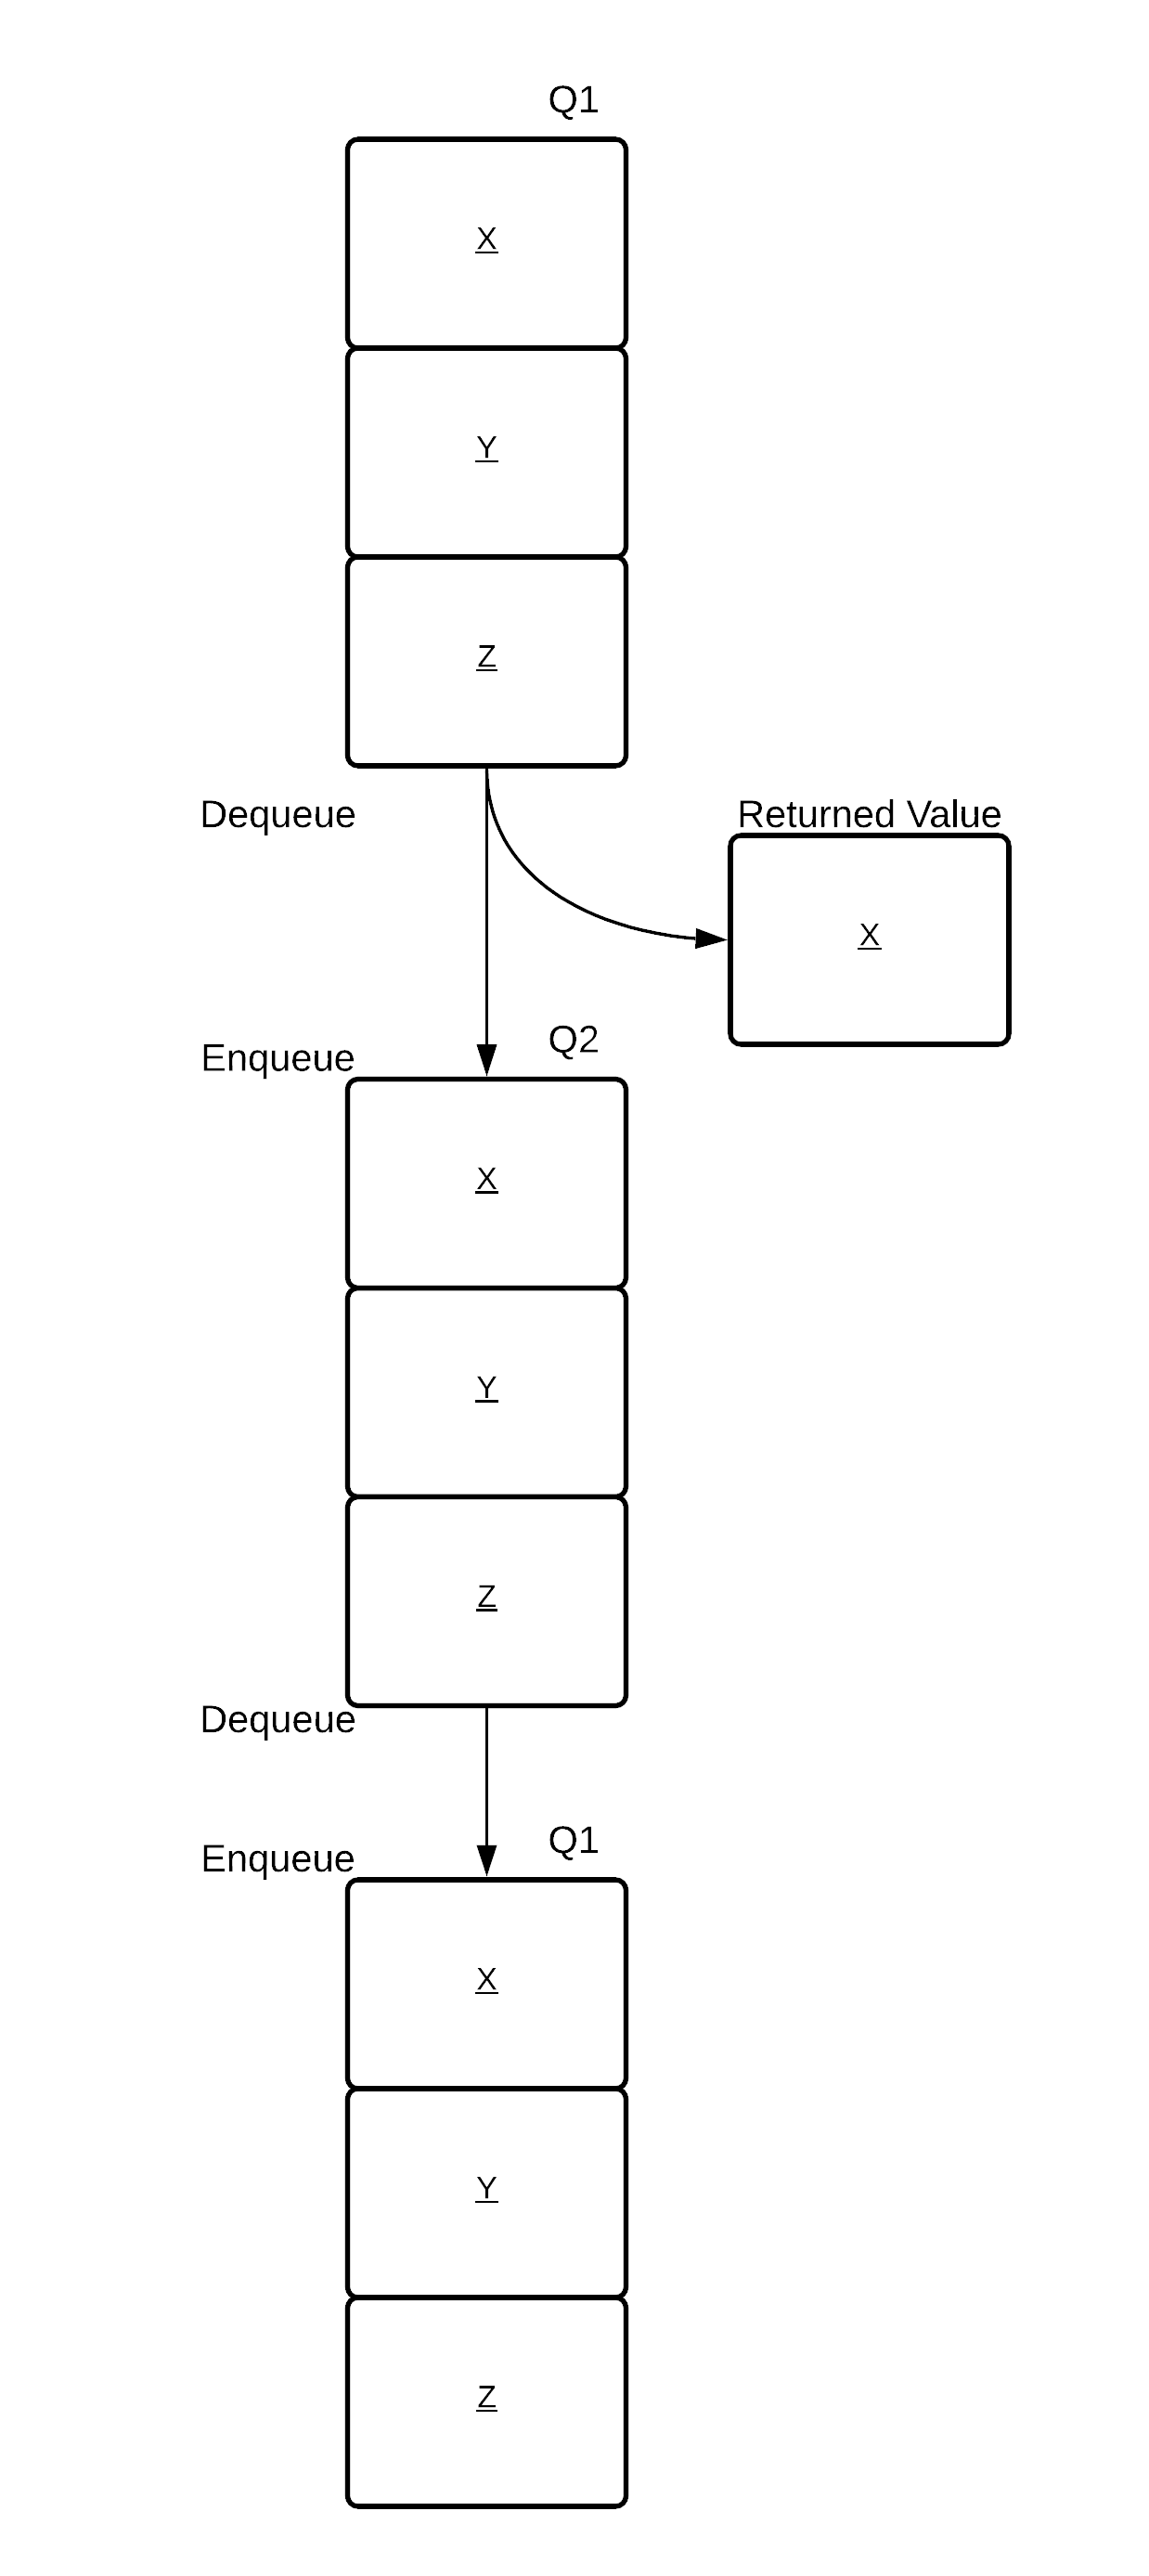
\includegraphics[scale = 0.17]{peek.png}
    \caption{peek() operation sequence.}
\end{figure}
\begin{figure}[H]
    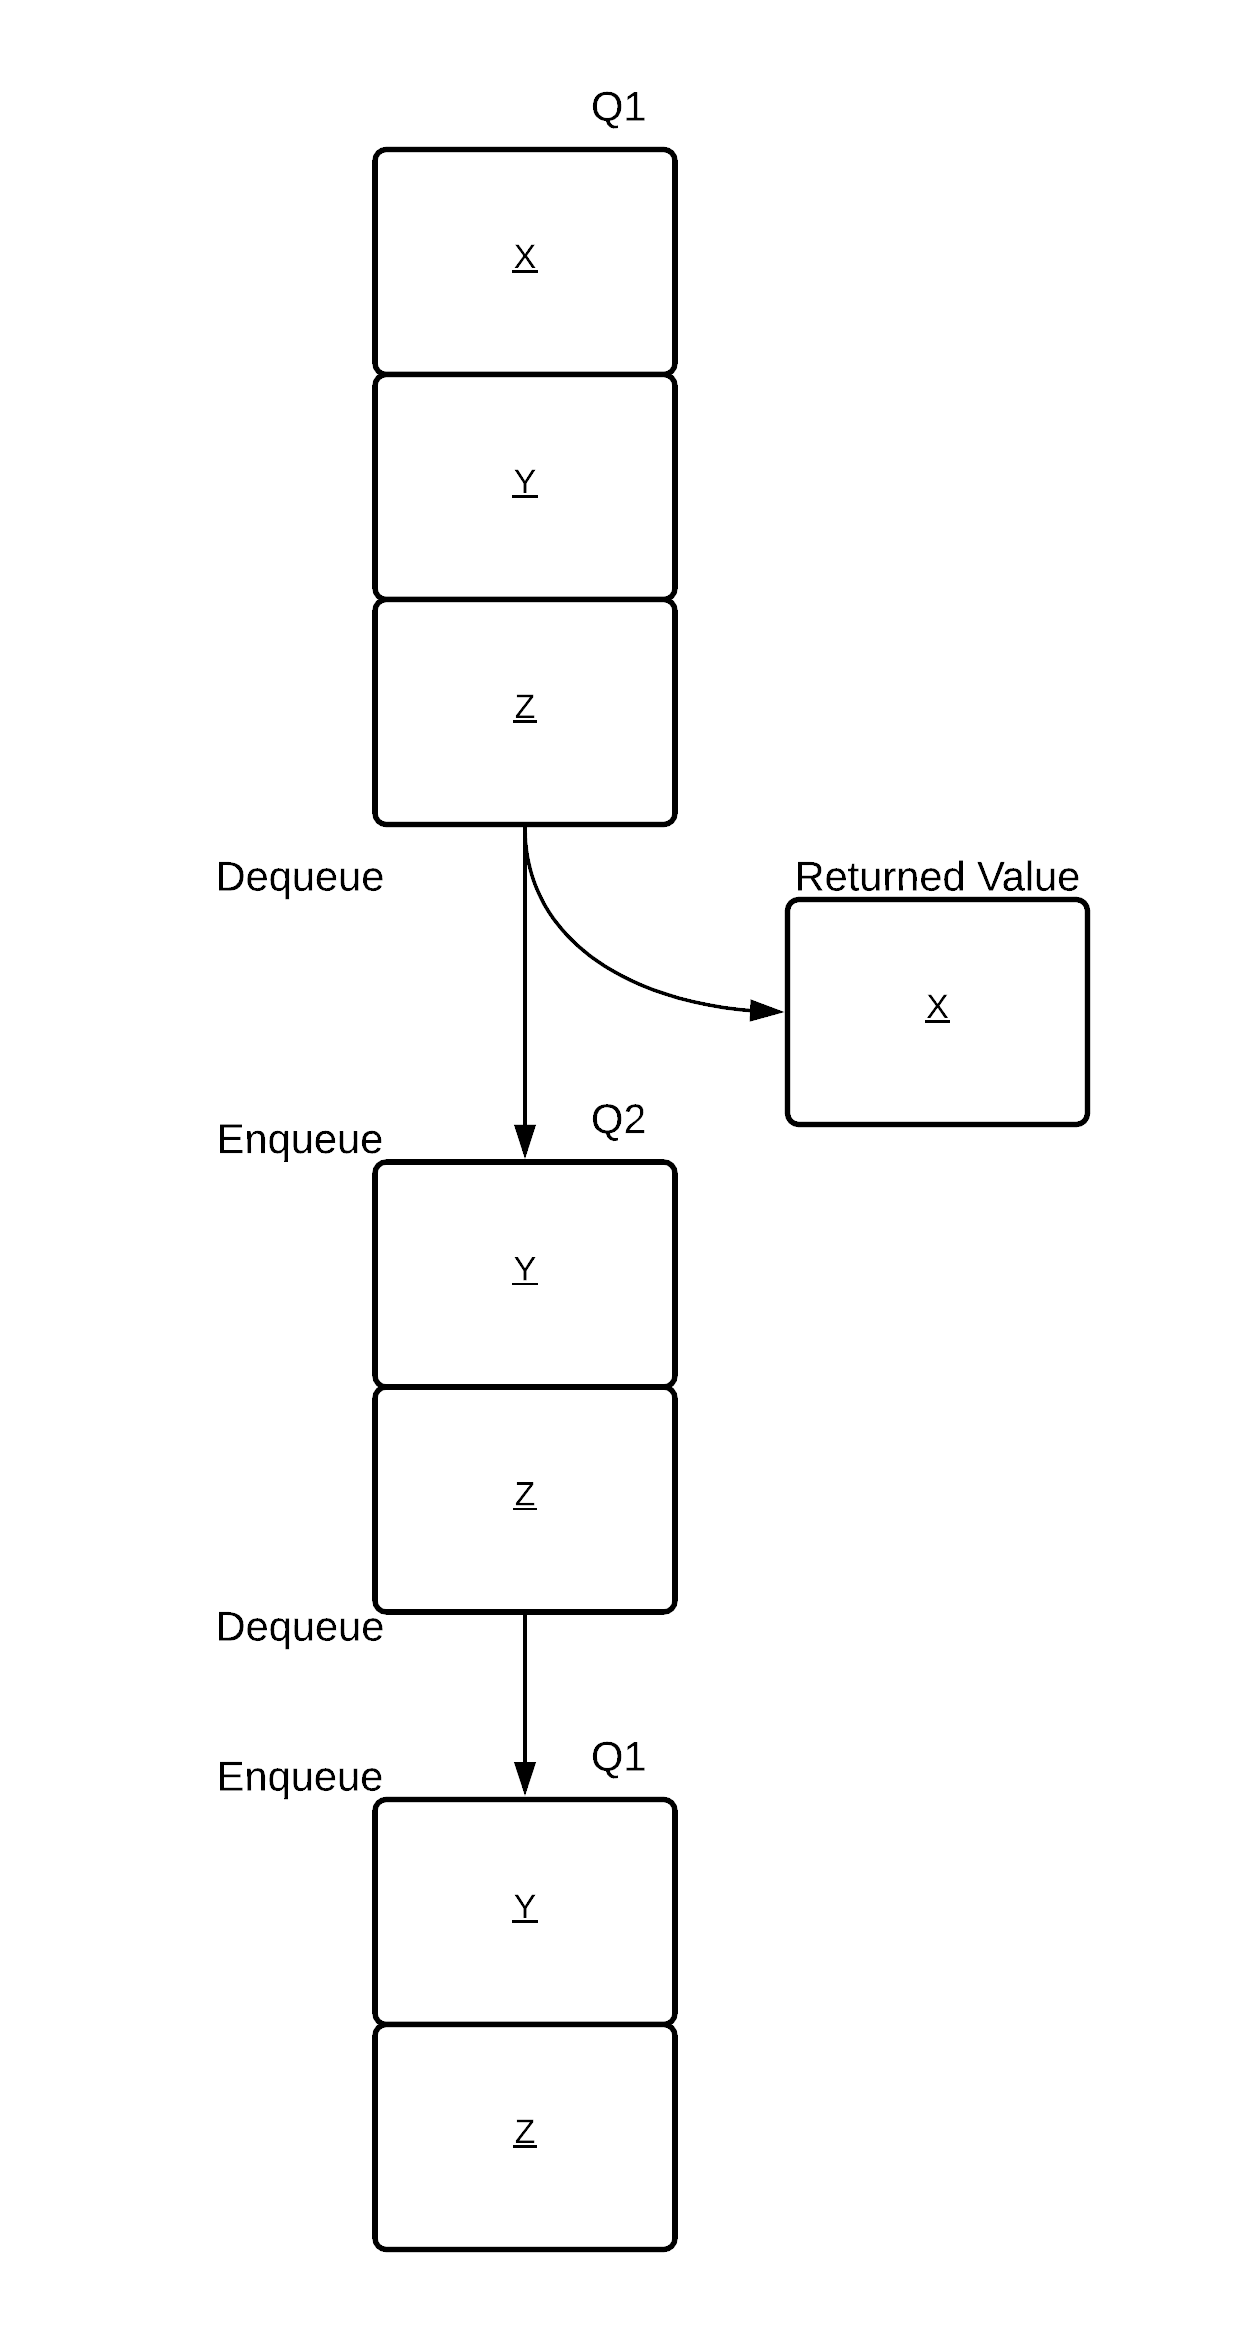
\includegraphics[scale = 0.17]{pop.png}
    \caption{pop() operation sequence.}
\end{figure}
\begin{figure}[H]
    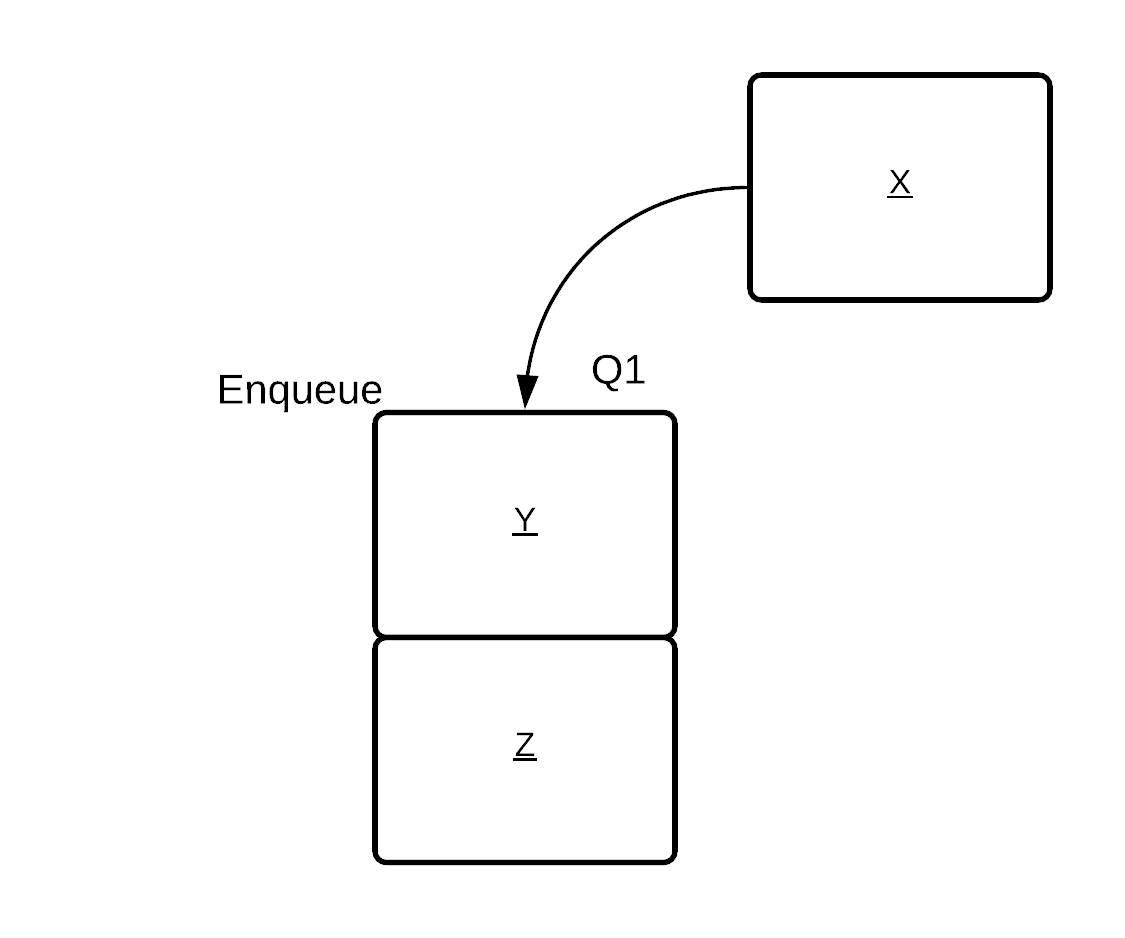
\includegraphics[scale = 0.17]{push.png}
    \caption{push() operation sequence.}
\end{figure}

\begin{algorithm}
    \caption{Object peek()}
    \begin{algorithmic}
        \REQUIRE{$Q1, Q2$}
        \STATE $initialize~temp = 0:~O(1)$
        \STATE $initialize~return~object = 0:~O(1)$
        \FOR{$i = 0~\TO~Q1 \rightarrow size() - 1:~O(N)$}
        \STATE $Q1 \rightarrow dequeue \rightarrow temp:~O(1)$
        \IF{$i = Q1 \rightarrow size() - 1$}
        \STATE $temp \rightarrow return~object:~O(1)$
        \ENDIF
        \STATE $Q2 \rightarrow enqueue \rightarrow temp:~O(1)$
        
        \ENDFOR
        \FOR{$i = 0~\TO~Q2 \rightarrow size() - 1:~O(N)$}
        \STATE $Q2 \rightarrow dequeue \rightarrow temp:~O(1)$
        \STATE $Q1 \rightarrow enqueue \rightarrow temp:~O(1)$
        \ENDFOR
        \RETURN $return~object$
    \end{algorithmic}
\end{algorithm}

Total runtime of $peek()$ would be 
$$O(1) + O(1) + 3O(N)O(1) + 2O(N)O(1)$$
$$lim_{N \rightarrow \infty}2O(1) + 5O(N) \rightarrow O(N)$$

$\therefore peek() \in \boxed{O(N)}$.

\begin{algorithm}
    \caption{Object pop()}
    \begin{algorithmic}
        \REQUIRE{$Q1, Q2$}
        \STATE $initialize~temp = 0:~O(1)$
        \STATE $initialize~return~object = 0:~O(1)$
        \FOR{$i = 0~\TO~Q1 \rightarrow size() - 1:~O(N)$}
        \IF{$i = Q1 \rightarrow size() - 1$}
        \STATE $Q1 \rightarrow dequeue \rightarrow return~object:~O(1)$
        \STATE $break~loop$
        \ENDIF
        \STATE $Q1 \rightarrow dequeue \rightarrow temp:~O(1)$
        
        \STATE $Q2 \rightarrow enqueue \rightarrow temp:~O(1)$
        \ENDFOR
        \FOR{$i = 0~\TO~Q2 \rightarrow size() - 1:~O(N)$}
        \STATE $Q2 \rightarrow dequeue \rightarrow temp:~O(1)$
        \STATE $Q1 \rightarrow enqueue \rightarrow temp:~O(1)$
        \ENDFOR
        \RETURN $return~object$
    \end{algorithmic}
\end{algorithm}

Total runtime of $pop()$ would be 
$$O(1) + O(1) + 3O(N)O(1) + 2O(N)O(1)$$
$$lim_{N \rightarrow \infty}2O(1) + 5O(N) \rightarrow O(N)$$

$\therefore peek() \in \boxed{O(N)}$.

\begin{algorithm}
    \caption{void push()}
    \begin{algorithmic}
        \REQUIRE{$Q1, value~to~push~(X)$}
        \STATE $Q1 \rightarrow enqueue \rightarrow X:~O(1)$
    \end{algorithmic}
\end{algorithm}

Total runtime of $push()$ would be 
$$lim_{N \rightarrow \infty}O(1) \rightarrow O(1)$$

$\therefore push() \in \boxed{O(1)}$.




\end{document}
